\documentclass[a4paper]{article}
\usepackage[UTF8]{ctex}
\usepackage{geometry}
\usepackage{graphicx}
\usepackage{url}
\usepackage{multirow}
\usepackage{array}
\usepackage{booktabs}
\usepackage{url}
\usepackage{enumitem}
\usepackage{graphicx}
\usepackage{float}
\usepackage{amssymb}
\usepackage{amsmath}
\usepackage{subfig}
\usepackage{longtable}
\usepackage{pifont}
\usepackage{color}

\allowdisplaybreaks

\geometry{a4paper, scale=0.78}

% \begin{figure}[H]
%     \centering
%     \includegraphics[width=.55\textwidth]{E.png}
%     \caption{矩阵与列向量的乘法}
%     \label{fig:my_label_1}
% \end{figure}

% \left\{
% \begin{array}{ll}
%       x+2x+z=2 & \\
%       3x+8y+z=12 & \\
%       4y+z=2
% \end{array}
% \right.

% \begin{enumerate}[itemindent = 1em, itemsep = 0.4pt, parsep=0.5pt, topsep = 0.5pt]

% \end{enumerate}

%\stackrel{a}{\longrightarrow}

\title{Support Vector Machine 04 Weak Duality Geometric Interpretation}
\author{Chen Gong}
\date{17 November 2019}

\begin{document}
\maketitle
上一小节中我们讨论了有关弱对偶性的证明,这一节我们从几何的角度来解释一下有关对偶问题。为了方便描述,我们将对偶问题进行简化为如下形式:
\begin{equation}
    \left\{
    \begin{array}{ll}
        \min_{x\in \mathcal{R}^p} \ f(x) & \\
        s.t. \quad m_i \leq 0 & \\
    \end{array}
    \right.
\end{equation}

$\mathbb{D}:$定义域,$D=dom\ f \cap dom\ m_i$,这是一种常见的定义域的表示方法。其中,$x\in \mathbb{D}$。我们将模型表达为拉格朗日函数的形式,
\begin{equation}
    \mathcal{L}(x,\lambda) = f(x) + \lambda m_1(x),\qquad \lambda \leq 0
\end{equation}

我们将原问题的最优解记为:$p^\ast = \min\ f(x)$。

我们将对偶问题的最优解记为:$d^\ast = \max_{\lambda} \min_{x} \ \mathcal{L}(x,\lambda)$。

\section{模型表述}
上述表述中,表达了模型的基本问题,下面我们进一步抽象模型。首先,我们需要描述一个集合:
\begin{equation}
    G = \{ (m_1(x),f(x))|x \in \mathbb{D} \}
\end{equation}

为了简化运算,我们需要简化符号,令$m_1(x) = \mu,\ f(x)=t$。那么,
\begin{equation}
    G = \{ (\mu,t)|x \in \mathbb{D} \}
\end{equation}

我们需要想想如何集合话来表示,首先$p^\ast = \min \ f(x) = \min \ t$,其中,$\left\{ t|(\mu,t)\in G \right\}$。那么,我们用$inf$来表示下确界的意思,就有:
\begin{equation}
    p^\ast = inf\left\{ t|(\mu,t)\in G,\mu \leq 0 \right\}
\end{equation}

那么对偶问题,我们可以写成,
\begin{equation}
    d^\ast = \max_{\lambda}\min_{x} \ \mathcal{L}(x,\lambda)=\max_{\lambda}\min_{x} (t+\lambda \mu)
\end{equation}

又因为$(t+\lambda \mu)$只和$\lambda$有关,那么可以被记做$g(\lambda)$。而且,$g(\lambda)$可以被写作,$g(\lambda) = inf (t+\lambda \mu)|(\mu,t)\in G$。在对偶条件中不需要那个$\mu \leq 0$,因为已经包含在原等式的隐藏条件里了。但是,在原问题中,我们一定不能忘记这个条件。

\section{模型表达}
\subsection{$p^\ast$的几何表示}
下一步的主要问题就是,我们需要如何来表达$p^\ast$和$d^\ast(g(\lambda))$。首先我们来看$p^\ast$,其实它的表达还算比较简单。我们来看这个图像的表达式:
\begin{figure}[H]
    \centering
    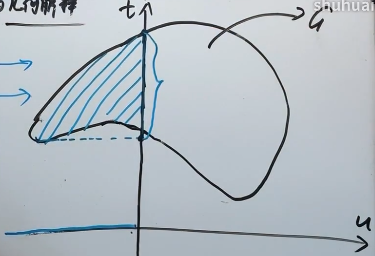
\includegraphics[width=.45\textwidth]{微信图片_20191117141212.png}
    \caption{$p^\ast$的几何表示}
    \label{fig:my_label_1}
\end{figure}

我们假设G就是$(\mu,t)$的定义域的几何表示区间。$p^\ast = inf\left\{ t|(\mu,t)\in G,\mu \leq 0 \right\}$,由于$\mu \leq 0$,所以我们只看左边一半。那么$t$的值就是坐标纵轴上的一截部分。最小值非常的好确定,就是平行于$\mu$轴,最下方的切点。

\subsection{$d^\ast(g(\lambda))$的几何表示}
这个等式的几何表示就会有点困难了,我们需要分解成两步,第一步确定$g(\lambda)$的几何表达;第二步,确定$d^\ast$的几何表达。

\subsubsection{$g(\lambda)$的几何表达}
由于$t+\lambda \mu$是一个关于x的变量,在这其中$\lambda$起到的是一个斜率的作用,这个斜率是一直保持不变的。而得到的$t+\lambda \mu$的结果我们记为$\triangle$。$\triangle$也就是$t+\lambda \mu$和t轴的交点。那么,也就是一根固定斜率的直线在t的方向上进行移动。
\begin{figure}[H]
    \centering
    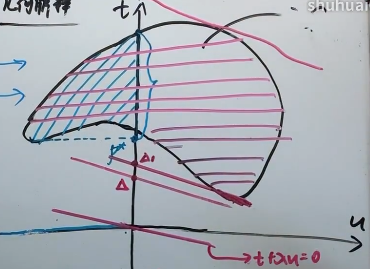
\includegraphics[width=.4\textwidth]{微信图片_20191117143523.png}
    \caption{$g(\lambda)$的几何表达}
    \label{fig:my_label_1}
\end{figure}

我们可以假设$t+\lambda \mu$与t轴的交点是一个集合,这个集合就是$\{\triangle_1,\triangle_2,\cdots,\triangle_N\}$。

\subsubsection{$d^\ast$的几何表达}
下一步,我们需要求的是$d^\ast = \max_{\lambda} g(\lambda)$。现在相当于是固定了一个点,然后围着这个点在转。这个点是哪个店呢?就是$(0,t)$。大家仔细想一想比对一下上图就知道是不是转到与集合$G$相切的时候得到的这个解是最优解,但是这个解一定会比$p^\ast$得到的解会更小。为什么?用屁股想都知道,一个是横着切,一个是斜着切,哪个会更小?不言而喻了吧。通过这个我们也可以得到,
\begin{equation}
    d^\ast \leq p^\ast
\end{equation}

\section{小结}
上面我们从几何的角度来重新解释了这个问题,其实仔细的想一想也不算很难。但是,强对偶性的证明这个东西有点难,实际上学习机器学习中的SVM,学到这就差不多够了。如果是强对偶性,我们还需要满足两个条件,也就是1. 是一个凸优化问题;2. slate条件。就可以得到$d^\ast = p^\ast$。下一节会进一步解释,但是这只是一个充分必要条件,满足其他的条件也可能是强对偶关系。而SVM是一个二次规划问题,那么它一定是一个强对偶问题。





\end{document}
